\documentclass[10pt,aspectratio=43,mathserif,table]{beamer} 
%  设置为 Beamer 文档类型,设置字体为 10pt,长宽比为16:9,数学字体为 serif 风格
\batchmode
\usepackage{graphicx}
\usepackage{subfigure}
\usepackage{fontspec}

\setmainfont{Harding Text Web Regular Regular.ttf}
\usepackage{diagbox} % 表头斜线分区
\usepackage{unicode-math}
\usefonttheme{serif}
\setmathrm{Harding Text Web Regular Regular.ttf} % 设置数学字体为 Times New Roman
\setmathfont{TeX Gyre Termes Math} % 如果您使用 XeLaTeX 或 LuaLaTeX 编译,可以使用其他数学字体
\setmathtt{Courier New} % 设置等宽字体为 Courier New
\setboldmathrm{Times New Roman}
\setmathfont{TeX Gyre Termes Math}[version=bold] % 设置粗体数学字体
\setmathfont{TeX Gyre Termes Math}[range={\mathit}]


\usetheme{Berlin} %主题
\setbeamertemplate{page number in head/foot}[pagenumber]
%\usecolortheme{sustech} %主题颜色

\usepackage[ruled,linesnumbered]{algorithm2e}

\usepackage{fancybox}
\usepackage{xcolor}
\usepackage{listings}

\usepackage{booktabs}
\usepackage{colortbl}

\newcommand{\Console}{Console}
\lstset{ %
	backgroundcolor=\color{white},   % choose the background color
	basicstyle=\footnotesize\rmfamily,     % size of fonts used for the code
	columns=fullflexible,
	breaklines=true,                 % automatic line breaking only at whitespace
	captionpos=b,                    % sets the caption-position to bottom
	tabsize=4,
	commentstyle=\color{mygreen},    % comment style
	escapeinside={\%*}{*)},          % if you want to add LaTeX within your code
	keywordstyle=\color{blue},       % keyword style
	stringstyle=\color{mymauve}\ttfamily,     % string literal style
	numbers=left, 
	%	frame=single,
	rulesepcolor=\color{red!20!green!20!blue!20},
	% identifierstyle=\color{red},
	language=c
}


\definecolor{mygreen}{rgb}{0,0.6,0}
\definecolor{mymauve}{rgb}{0.58,0,0.82}
\definecolor{mygray}{gray}{.9}
\definecolor{mypink}{rgb}{.99,.91,.95}
\definecolor{mycyan}{cmyk}{.3,0,0,0}

%题目,作者,学校,日期
\title{Paper Reading}
%\subtitle{\fontsize{9pt}{14pt}\textbf{跨临界分岔}}
\author{Speaker: Yichen Lu\quad \newline  \newline \quad }
\institute{\fontsize{8pt}{14pt}}
\date{\today}
\newcommand{\concept}{Paper Reading}

%学校Logo
%\pgfdeclareimage[height=0.5cm]{sustech-logo}{sustech-logo.pdf}
%\logo{\pgfuseimage{sustech-logo}\hspace*{0.3cm}}

\AtBeginSection[]
{
	\begin{frame}<beamer>
	\frametitle{\textbf{Contents}}
	\tableofcontents[currentsection]
\end{frame}
}
% \beamerdefaultoverlayspecification{<+->}
% -----------------------------------------------------------------------------
\begin{document}

\section{Chen Y, 2014}

\begin{frame}
	\begin{figure}
		\centering
		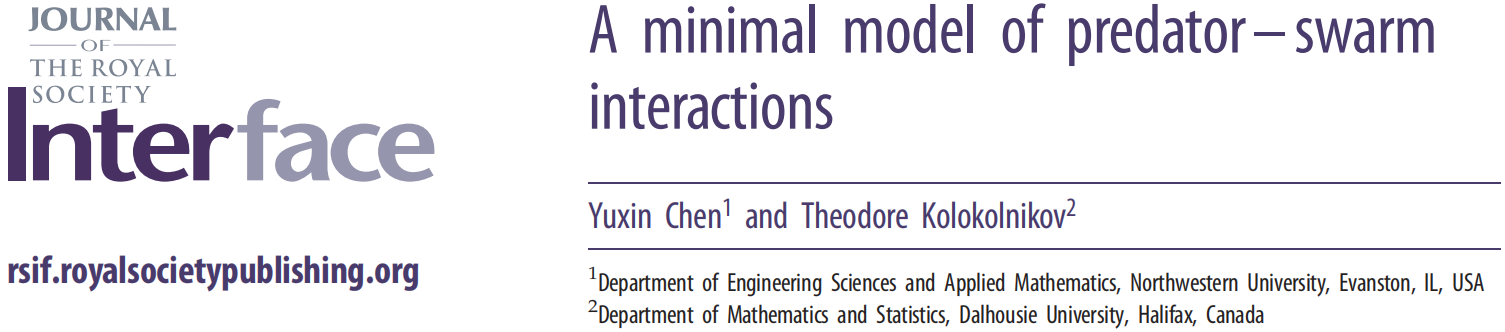
\includegraphics[width=\textwidth]{ChenY2014Face.jpg}
	\end{figure}
	
	\textbf{Keywords:}  predator–prey interactions, biological, aggregation, dynamical systems
\end{frame}

\begin{frame}
    The model of this paper:
	$$
	\frac{dx_j}{dt}=\frac{1}{N}\sum_{k=1,k\ne j}^N{\left( \frac{x_j-x_k}{\left| x_j-x_k \right|^2}-a\left( x_j-x_k \right) \right) +b\frac{x_j-z}{\left| x_j-z \right|^2}}
	$$
	and
	$$
	\frac{dz}{dt}=\frac{c}{N}\sum_{k=1}^N{\frac{x_k-z}{\left| x_k-z \right|^p}}
	$$
\end{frame}

\section{My Model}

\begin{frame}
    $$
    \dot{\mathrm{x}}_i=\frac{1}{N}\sum_{\begin{array}{c}
        j=1\\
        j\ne i\\
    \end{array}}^N{\left[ \frac{\mathrm{x}_j-\mathrm{x}_i}{\left| \mathrm{x}_j-\mathrm{x}_i \right|}\left( 1+J\cos \left( \theta _j-\theta _i \right) \right) -\frac{\mathrm{x}_j-\mathrm{x}_i}{\left| \mathrm{x}_j-\mathrm{x}_i \right|^2} \right]}-F\frac{\mathrm{x}_0-\mathrm{x}_i}{\left| \mathrm{x}_0-\mathrm{x}_i \right|^2}
    $$

    $$
    \dot{\theta}_i=\frac{K}{N}\sum_{\begin{array}{c}
        j=1\\
        j\ne i\\
    \end{array}}^N{\frac{\sin \left( \theta _j-\theta _i \right)}{\left| \mathrm{x}_j-\mathrm{x}_i \right|}}
    $$

	$$
	\dot{\mathrm{x}}_0=\frac{c}{N}\sum_{k=1}^N{\frac{\mathrm{x}_i-\mathrm{x}_0}{\left| \mathrm{x}_i-\mathrm{x}_0 \right|^p}}
	$$

\end{frame}



% -----------------------------------------------------------------------------
\end{document}
